% 独自のコマンド

% ■ アブストラクト
%	\begin{jabstract} ~ \end{jabstract}	:日本語のアブストラクト

% ■ 謝辞
%	\begin{acknowledgment} ~ \end{acknowledgment}

% ■ 文献リスト
%	\begin{bib}[100] ~ \end{bib}

% styファイルは同ディレクトリにおいておけば,latexmkrcの設定をいじらなくても上手くいくらしい
\newif\ifjapanese

\japanesetrue	% 論文全体を日本語で書く(英語で書くならコメントアウト)

\ifjapanese
	\documentclass[12pt]{jreport}
	\renewcommand{\bibname}{参考文献}
	\newcommand{\acknowledgmentname}{謝辞}
\else
	\documentclass[11pt]{report}
	\newcommand{\acknowledgmentname}{Acknowledgment}
\fi
\usepackage{ascmac}
\usepackage[dvipdfmx]{graphicx}
\usepackage{multirow}
\usepackage{ylab_thesis} % このスタイルファイルが同じディレクトリにあることを確認すること
\usepackage{layout}

% \documentclass[dvipdfmx]{jsarticle}
% \usepackage[dvipdfmx]{graphicx}
\usepackage{amsmath, amssymb}
\usepackage{mathtools}
\usepackage{here}

% \bindermode	% バインダ用余白設定

% 日本語情報(必要なら)
\jclass	{卒業論文}							% 論文種別
\jtitle		{オープンセット環境下におけるレーダ心拍信号を用いた深層学習による人物識別}					% タイトル。改行する場合は\\を入れる
\juniv		{慶 應 義 塾 大 学}					% 大学名
\jfaculty	{理 工 学 部 情 報 工 学 科}				% 学部、学科
\jlab		{大 槻 研 究 室}						% 研究室
\jauthor	{権 藤 陸}						% 著者
\jid		{61908013}						% 学籍番号
\jadvisor	{大 槻 知 明}{教 授}					% 指導教官、形式は『{名前}{肩書}』
\jsubmit	{令和 5 年 2 月 3 日}
\jhyear		{5}							% 平成○年度
\jsyear		{2023}							% 西暦○年度
\jkeyword	{キーワード1,キーワード2,キーワード3}		% 論文のキーワード


\begin{document}

\jmaketitle		% 表紙(日本語)、不要ならコメントアウト

%%% アブストラクト
\begin{jabstract}

テンプレートの説明を,テンプレート自身を使って説明する.これは卒業論文のための\LaTeX テンプレートで,本当は卒業論文のために作成したものだけどでもたぶんきっと修士論文にも使えると思う.

この部分には一般には論文のアブストラクトを書く.日本語のアブストラクトを書きたいなら,\verb|\begin{jabstract}| と \verb|\end{jabstract}| の間に文章を書けば,今のこのページのように体裁が勝手に整って出力される.英語のアブストラクトは \verb|\begin{eabstract}| と \verb|\end{eabstract}| の間に書けば,次ページのような体裁で出力される.

両方を書けば,日本語と英語の両方のアブストラクトが並んで出力される(この文書はサンブルなので両方書いてある).ページ順序は,コマンドを書いた順序の通り.どちらか一方のみを出力したい場合は,不要な方をコマンド自体を含め削除する.

このあたりの詳細もあとで書く.基本的には,{\tt main.tex}を上から順にいじっていけばできるはず.

(2018/11 中村追記) ファイル分割を廃止し{\tt main.tex}に統一している.

\end{jabstract}

\tableofcontents	% 目次
\listoffigures		% 表目次
\listoftables		% 図目次

\pagenumbering{arabic}

\chapter{序論}
\label{chap_introduction}

論文は序論のようなもので始める.タイトルは序論でも序言でもはじめにでもいいけど,『序論』で始めたら『結論』で終わり,『序言』で始めたら『結言』で終わるようにする.『はじめに』なら『おわりに』で終わる.『序論』で始まって『おわりに』でおわるとか,そういうちぐはぐなのはだ.

ここでは序論として書く.序論では,研究の背景やら目的やらを書くのが普通.今はテンプレートの説明なので,大して書くことは無い.

このような高齢者の家庭内事故の現状を踏まえると,高齢者が最も遭遇しやすい事故は屋内での転倒・転落事故と推定され,
これらの異常事態の迅速かつ高精度な検知が今後の見守りシステムにおける重要課題と言える.

\section{背景}

卒論向けテンプレ

\section{本文書の構成}

第1章の最後は,文書全体の構成を大まかに書くとよいらしい.

第\ref{chap_introduction}章では本テンプレートの概要みたいなものを書いた.



\chapter{ドップラーレーダの原理}
\begin{equation*} f_{\mathrm{ Doppler}} = \mp \frac {4 \pi vt}{\lambda } \times \frac {1}{2 \pi t} = \mp \frac {2v}{\lambda },\tag{1}\end{equation*}

\begin{equation*} B(t)=\cos \left({\theta +\frac {4\pi x_{h}(t)}{\lambda }+\Delta \Phi (t)}\right),\tag{2}\end{equation*}

\begin{align*} I(t)=&\cos \left({\theta +\frac {\pi }{4}+\frac {4\pi x_{h}(t)}{\lambda }+\Delta \Phi (t)}\right), \tag{3}\\ Q(t)=&\cos \left({\theta -\frac {\pi }{4}+\frac {4\pi x_{h}(t)}{\lambda }+\Delta \Phi (t)}\right).\tag{4}\end{align*}

\chapter{関連研究}

\chapter{従来法}

\chapter{提案法}
提案法のアルゴリズムを図\ref{fig:proposed_method}に示す.
本提案では,6ポートのドップラーレーダで取得したI/Qデータを用いた.
I/Qデータには心拍信号や呼吸信号に起因する胸壁の変位以外に,体動などの外乱ノイズやレーダのキャリブレーションによるノイズが含まれている.

\begin{figure}[H]
\begin{center}
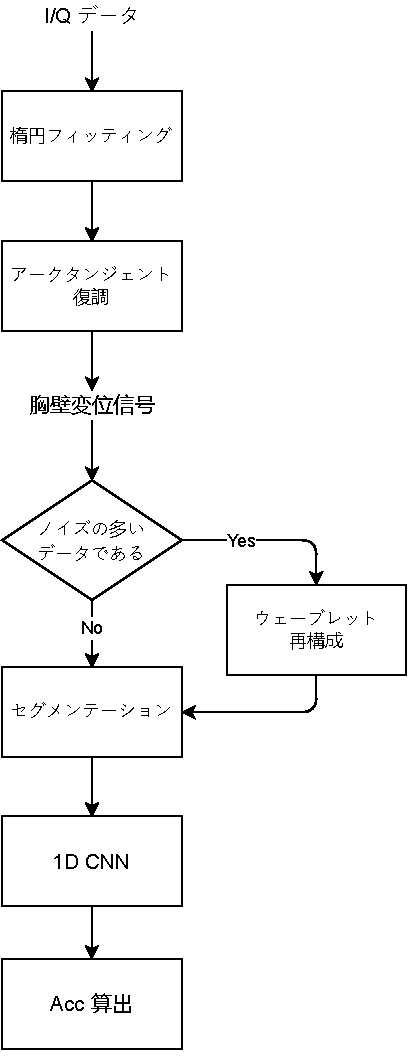
\includegraphics[width=0.5\linewidth]{./fig/proposed_method.pdf}
\end{center}
\caption{提案法のアルゴリズム}
\label{fig:proposed_method}
\end{figure}

\chapter{結論}

\chapter{それ以降の書き方}
\section{構成}
基本的に,以下のような流れになるが,これに従う必要はない.
おそらく{\tt subsection}や{\tt subsubsection}でまとめる場合もあるはず.

\begin{enumerate}
	\item 序論
	\item 関連研究
	\item 従来法
	\item 提案法
	\item 実験・評価
	\item 考察
	\item 結論
	\item 参考文献
\end{enumerate}

わからなければ,今までサーベイした国際会議の論文や,先輩の卒業論文を参考にしよう.
分量としては,一般的な国内研究会・国際会議のスタイル (2カラム10ポイント) で5・6枚程度の論文の場合,卒論のスタイルファイルに当てはめると40枚超にはなるはず.

\section{参考文献について}
このテンプレ中では{\tt thebibliography}を使用しているが,BibTexのほうが使いやすいと思う場合は変更すること.
引用フォーマットに関しては,IEEEのフォーマット{\tt IEEETran}に筆者は合わせた.

% 謝辞
\begin{acknowledgment}

謝辞には,お世話になった先生,先輩,後輩,友人など,感謝の気持ちを書く.論文が『である』調でも,謝辞だけは『ですます』調で書くひともいる.

\end{acknowledgment}

% 参考文献
\begin{bib}[100]

% \bibitem{参照用名称}
%   著者名: 
%   \newblock 文献名,
%   \newblock 書誌情報,出版年.

\bibitem{hoge09}
  ほげ山太郎,ほげ山次郎:
  \newblock ほげほげ理論のHCI分野への応用,
  \newblock ほげほげ学会論文誌,Vol.31,No.3,pp.194-201,2009.

\bibitem{hoge08}
  Taro Hogeyama, Jiro Hogeyama:
  \newblock The Theory of Hoge,
  \newblock {\it The Proceedings of The Hoge Society}, 2008.
	
\end{bib}

\appendix
% 付録
\chapter{付録の例}

付録を無理矢理出力させるため,てきとうなことを書く

\section{付録1}

コマンドは本文と一緒.

\subsection{あの}

あのイーハトーヴォのすきとおった風,夏でも底に冷たさをもつ青いそら,うつくしい森で飾られたモリーオ市,郊外のぎらぎらひかる草の波.

\section{なにか}

あのイーハトーヴォのすきとおった風,夏でも底に冷たさをもつ青いそら,うつくしい森で飾られたモリーオ市,郊外のぎらぎらひかる草の波.

\subsection{foo}

あのイーハトーヴォのすきとおった風,夏でも底に冷たさをもつ青いそら,うつくしい森で飾られたモリーオ市,郊外のぎらぎらひかる草の波.

\end{document}

